%COCOMO
\section{COCOMO Approach}
In this chapter, we use COCOMO II in order to understand the Effort and Estimation. 
\\Scale Drivers and Cost Drivers are deeply analysed here. They are needed for the calculate of the Effort Equation, the main COCOMO formula.
\\\begin{center} Effort = $A * EAF * KSLOC^E$  , where A = 2.94 . \end{center}
From the Scale Drivers, we obtain E, while from the Cost Drivers we obtain EM. 

\section{Scale Drivers}
We use the Scale Factors table to obtain the values associated with the five main factors that characterize our Scale Drivers. %PRODUCT
\begin{center}
\begin{figure}[!ht]
  \centering
  \vspace{0.2cm}
  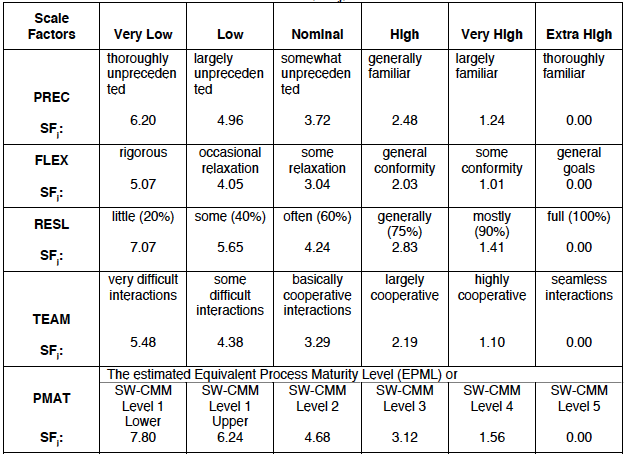
\includegraphics[width=1.0\textwidth]{/PP/Scale_factors}\\
  \vspace{0.2cm}
  %\caption{Mockup for the login mobile page} 
  \label{fig:scale_factors} 
\end{figure}
\end{center}

Now we firstly analyse this factors:
\begin{itemize}
    \item \textbf{Precedentedness}: this's the first project of this kind that our team developed. So, the value will be set low.
    \item \textbf{Development Flexibility}: there some instructions provided by the stakeholders but the specifics of the project are decided by us. Then, the value will be set high.
    \item \textbf{Architecture / Risk Resolution}: we have a good risk management plan, the architecture is well-define and the schedule is planned in an efficiency way. The value will be set very high. 
    \item \textbf{Team Cohesion}: we were able to work as a team, we shared the same vision and to work together, especially for planning each assignment and for check each document before the release. Then, also this value will be set very high.
    \item \textbf{Process Maturity}: the maturity of our Project is assessed by well know method, called CMMI, and can be evaluated as Quantitatively Managed. The value will be set nominal. 
\end{itemize}

\begin{center}
  \begin{tabular}{ l | l | l }% p{10cm} }
   	\hline
	\textbf{Scale Factor} & \textbf{Factor} & \textbf{Value}
   	\\ \hline
    Precedentedness & low & 4.96
    \\\hline
    Development Flexibility & high & 2.03
    \\\hline
    Architecture / Risk Resolution & high & 1.41
    \\\hline
    Team Cohesion & very high & 1.10
 	\\\hline
 	Process Maturity & nominal & 4.68
   	\\\hline 
  \end{tabular}
  \begin{tabular}{ l l | l }% p{10cm} }
   	\\\textbf{TOTAL} & & 14.18
  \end{tabular}
\end{center}

\subsection{Evaluation of the Exponent E}
The equation that we use for evaluationg the Evaluation of the Exponent is:
\\\\E = $B + 0.01 * \sum_{j=1}^{5} SF_j$ , where B = 0.91 .
\\\\For our project $E = 0.91 + 0.01 x 14.18 \cong $\textbf{1.052}

\newpage %SCEGLIERE SE USARE WE, US, OPPURE THE TEAM.
\section{Cost Drivers}
These are the 17 effort multipliers used in COCOMO® II Post-Architecture model to adjust the nominal effort, Person Months, to reflect the software product under development. They are grouped into four categories: product, platform, personnel, and project. From them we want to obtain the Effort Multiplier (EF).

\subsection{Product factors}
\begin{itemize}
    \item \textbf{Required Software Reliability (RELY)}: this is the measure of the extent to which the software must perform its intended function over a period of time. We can have high financial losses due to software failures, so the value will be set high.
    \begin{figure}[!ht]
      \centering
      \vspace{0.2cm}
      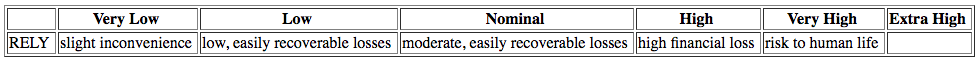
\includegraphics[width=1.0\textwidth]{/PP/Cost_drivers/RELY}\\
      \vspace{0.2cm}
      %\caption{Mockup for the login mobile page} 
      \label{fig:RELY} 
    \end{figure}
    \item \textbf{Data Base Size (DATA)}: we will have an high number of reservations, rides and payments but each of them need only a little amount of space. The value will be set nominal.
    \begin{figure}[!ht]
      \centering
      \vspace{0.2cm}
      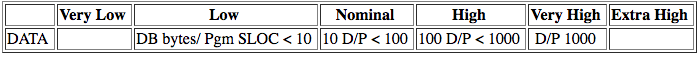
\includegraphics[width=1.0\textwidth]{/PP/Cost_drivers/DATA}\\
      \vspace{0.2cm}
      %\caption{Mockup for the login mobile page} 
      \label{fig:DATA} 
    \end{figure}
    \item \textbf{Product Complexity (CPLX)}: we have evaluated control operations, computational operations, device-dependent operations, data management operations, and user interface management operations main characteristics and performances. So, accordingly with the COCOMO® II CPLX rating scale the value will be set high.
	  \begin{figure}[!ht]
      \centering
      \vspace{0.2cm}
      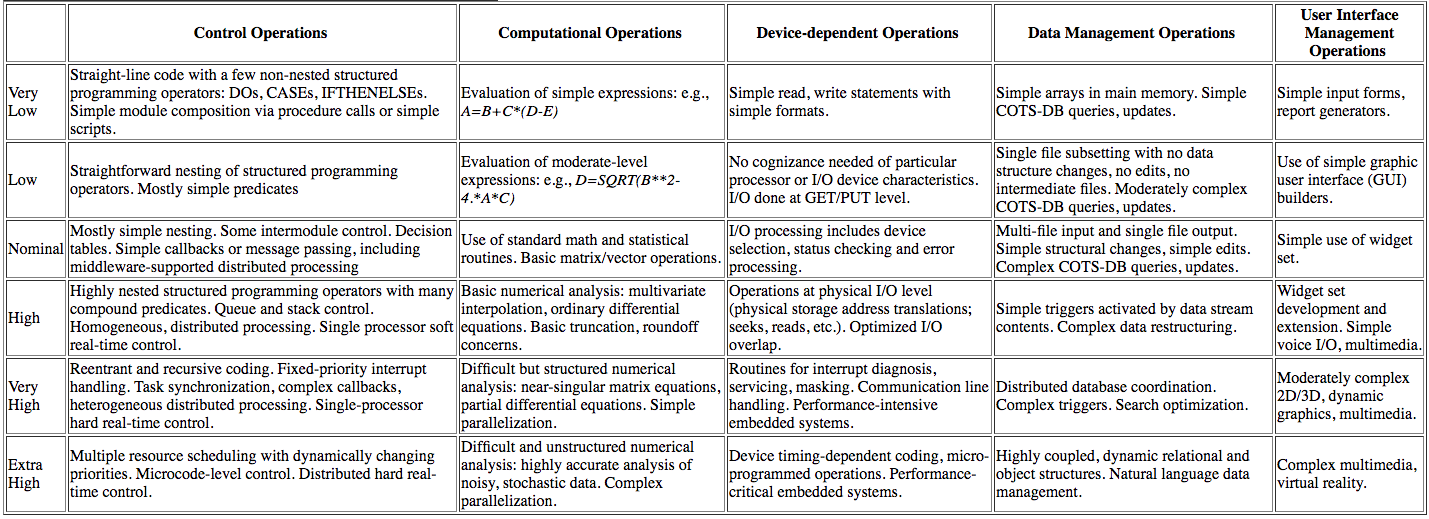
\includegraphics[width=1.2\textwidth]{/PP/Cost_drivers/CPLX}\\
      \vspace{0.2cm}
      %\caption{Mockup for the login mobile page} 
      \label{fig:CPLX} 
    \end{figure}
    \item \textbf{Developed for Reusability (RUSE)}: our efforts were aimed at the construction of components intended for reuse on the current or future projects. This effort is consumed with creating generic design of software, elaborate documentation, and extensive testing to ensure components are ready for use in other applications. Then, the value will be set high.
	   \begin{figure}[!ht]
      \centering
      \vspace{0.2cm}
      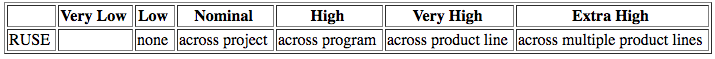
\includegraphics[width=1.0\textwidth]{/PP/Cost_drivers/RUSE}\\
      \vspace{0.2cm}
      %\caption{Mockup for the login mobile page} 
      \label{fig:RUSE} 
    \end{figure}
    \item \textbf{Documentation Match to Life-Cycle Needs (DOCU)}: the project's documentation is suitable with its life-cycle needs. The value for this cost driver will be set nominal.
    \begin{figure}[!ht]
      \centering
      \vspace{0.2cm}
      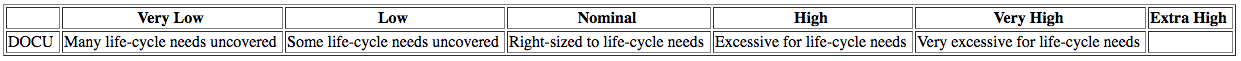
\includegraphics[width=1.0\textwidth]{/PP/Cost_drivers/DOCU}\\
      \vspace{0.2cm}
      %\caption{Mockup for the login mobile page} 
      \label{fig:DOCU} 
    \end{figure}
\end{itemize}

\subsection{Platform factors}
\begin{itemize}
    \item \textbf{Execution Time Constraint (TIME)}: the percentage of available execution time expected to be used by the system is quite low, less than 50\% of the execution time resource is consumed. So, the value will be set nominal.
    \begin{figure}[!ht]
      \centering
      \vspace{0.2cm}
      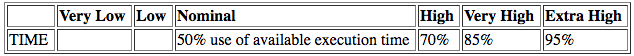
\includegraphics[width=1.0\textwidth]{/PP/Cost_drivers/TIME}\\
      \vspace{0.2cm}
      %\caption{Mockup for the login mobile page} 
      \label{fig:TIME} 
    \end{figure}
    \item \textbf{Main Storage Constraint (STOR)}: our project continue to expand with a low rate, and to consume whatever resources are available, making available processor execution time and main storage cost drivers still relevant. The value will be set nominal.
    \begin{figure}[!ht]
      \centering
      \vspace{0.2cm}
      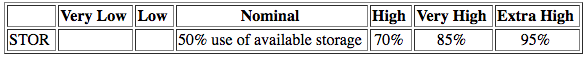
\includegraphics[width=1.0\textwidth]{/PP/Cost_drivers/STOR}\\
      \vspace{0.2cm}
      %\caption{Mockup for the login mobile page} 
      \label{fig:STOR} 
    \end{figure}
    \item \textbf{Platform Volatility (PVOL)}: we suppose that in our system there can be a major change every 6 months and a minor change every 2 weeks. These are maybe due to changes in the mobile operation systems or for the release of new and more performant software that we can use in the system. So, the value will be set nominal. 
    \begin{figure}[!ht]
      \centering
      \vspace{0.2cm}
      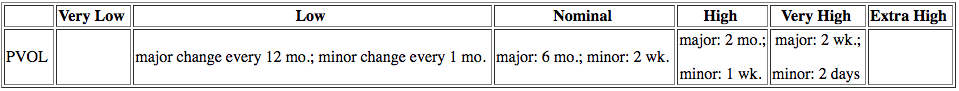
\includegraphics[width=1.0\textwidth]{/PP/Cost_drivers/PVOL}\\
      \vspace{0.2cm}
      %\caption{Mockup for the login mobile page} 
      \label{fig:PVOL} 
    \end{figure}
\end{itemize}

\subsection{Personnel Factors}
\begin{itemize}
    \item \textbf{Analyst Capability (ACAP)}: our Analysis and Design ability, efficiency and thoroughness, and the ability to communicate and cooperate, fall in the 75th percentile. Then, the value will be set high.
    \begin{figure}[!ht]
      \centering
      \vspace{0.2cm}
      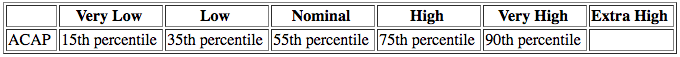
\includegraphics[width=1.0\textwidth]{/PP/Cost_drivers/ACAP}\\
      \vspace{0.2cm}
      %\caption{Mockup for the login mobile page} 
      \label{fig:ACAP} 
    \end{figure}   
    \item \textbf{Programmer Capability (PCAP)}: e didn't programme our application so we chose a medium value for not compromise the calculation. The value will be set nominal.
    \begin{figure}[!ht]
      \centering
      \vspace{0.2cm}
      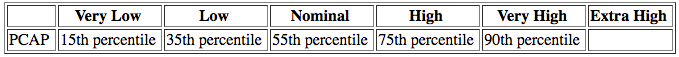
\includegraphics[width=1.0\textwidth]{/PP/Cost_drivers/PCAP}\\
      \vspace{0.2cm}
      %\caption{Mockup for the login mobile page} 
      \label{fig:PCAP} 
    \end{figure}   
    \item \textbf{Applications Experience (APEX)}:  Our level of experience with this type of application at the beginning of the project was very modest and then the value will be set low.
    \begin{figure}[!ht]
      \centering
      \vspace{0.2cm}
      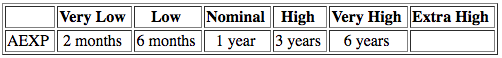
\includegraphics[width=1.0\textwidth]{/PP/Cost_drivers/APEX}\\
      \vspace{0.2cm}
      %\caption{Mockup for the login mobile page} 
      \label{fig:APEX} 
    \end{figure}   
    \item \textbf{Platform Experience (PLEX)}: our experience in recognize the importance of platforms, including more graphic user interface, database, networking, and distributed middleware capabilities is lower than six months. During other courses, we studied something useful here but most of the things were new for us and then the value will be set low.
    \begin{figure}[!ht]
      \centering
      \vspace{0.2cm}
      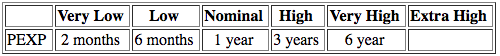
\includegraphics[width=1.0\textwidth]{/PP/Cost_drivers/PLEX}\\
      \vspace{0.2cm}
      %\caption{Mockup for the login mobile page} 
      \label{fig:PLEX} 
    \end{figure}  
    \item \textbf{Language and Tool Experience (LTEX)}: we had little experience with Latex and Draw.io, the two most important tools for our project. The value will be set nominal. 
    \begin{figure}[!ht]
      \centering
      \vspace{0.2cm}
      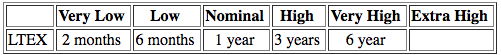
\includegraphics[width=1.0\textwidth]{/PP/Cost_drivers/LTEX}\\
      \vspace{0.2cm}
      %\caption{Mockup for the login mobile page} 
      \label{fig:LTEX} 
    \end{figure}  
    \item \textbf{Personnel Continuity (PCON)}: during the development of the project our team haven't got turnovers, so the value will be set very high.
    \begin{figure}[!ht]
      \centering
      \vspace{0.2cm}
      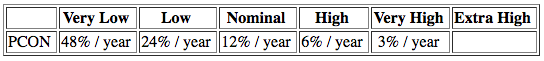
\includegraphics[width=1.0\textwidth]{/PP/Cost_drivers/PCON}\\
      \vspace{0.2cm}
      %\caption{Mockup for the login mobile page} 
      \label{fig:PCON} 
    \end{figure}  
\end{itemize}

\subsection{Project Factors}
\begin{itemize}
    \item \textbf{Use of Software Tools (TOOL)}: we used strong, mature lifecycle tools, moderately integrated. Then, the value will be set high.
     \begin{figure}[!ht]
      \centering
      \vspace{0.2cm}
      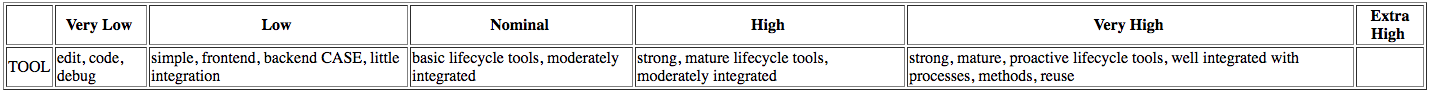
\includegraphics[width=1.0\textwidth]{/PP/Cost_drivers/TOOL}\\
      \vspace{0.2cm}
      %\caption{Mockup for the login mobile page} 
      \label{fig:TOOL} 
    \end{figure}  
    \item \textbf{Multisite Development (SITE)}: the project has an international distribution and has a full interactive multimedia access. The value will be set very high. 
     \begin{figure}[!ht]
      \centering
      \vspace{0.2cm}
      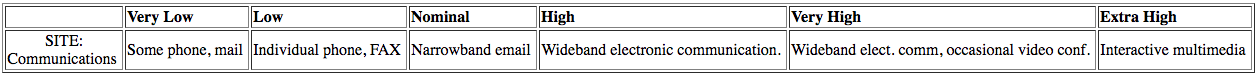
\includegraphics[width=1.0\textwidth]{/PP/Cost_drivers/SITE}\\
      \vspace{0.2cm}
      %\caption{Mockup for the login mobile page} 
      \label{fig:SITE} 
    \end{figure}  
\end{itemize}

\subsection{General Factor}
\begin{itemize}
    \item \textbf{Required Development Schedule (SCED)}: our schedule has been quite strict, the work had to be done on time so the stretch-out has been 100\% and the value will be set nominal.
    \begin{figure}[!ht]
      \centering
      \vspace{0.2cm}
      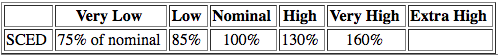
\includegraphics[width=1.0\textwidth]{/PP/Cost_drivers/SCED}\\
      \vspace{0.2cm}
      %\caption{Mockup for the login mobile page} 
      \label{fig:SCED} 
    \end{figure}
\end{itemize}


\begin{center}
  \begin{tabular}{ l | l | l }% p{10cm} }
   	\hline
	\textbf{Cost Driver} & \textbf{Factor} & \textbf{Value}
   	\\ \hline
    RELY & high & 1.15
    \\\hline
    DATA & nominal & 1.08
    \\\hline
    CPLX & high & 1.15
    \\\hline
    RUSE &  high & 1.15
 	  \\\hline
  	DOCU  & nominal & 1.00
   	\\\hline 
    TIME  & nominal & 1.00
   	\\\hline 
   	STOR  & nominal & 1.00
   	\\\hline 
   	PVOL  & nominal & 1.00
   	\\\hline 
   	ACAP  & high & 0.86
   	\\\hline 
   	PCAP  & nominal & 1.00
   	\\\hline 
   	APEX  & low & 1.10
   	\\\hline 
   	PLEX  & low & 1.10
   	\\\hline 
   	LTEX  & nominal & 1.00
   	\\\hline 
   	PCON  & very high & 0.65
   	\\\hline 
   	TOOL  & high & 0.91
   	\\\hline 
   	SITE  & very high & 0.86
   	\\\hline 
   	SCED  & nominal& 1.00
   	\\\hline 
  \end{tabular}
  \\\begin{tabular}{ l l | l }% p{10cm} }
   	\\\textbf{EAF} & & 1.356
  \end{tabular}
\end{center}

The EAF value is evaluated as: 
\\\begin{center}EAF = $\prod_{i=1}^{17} cost\_driver_i$ \end{center}

\section{Effort Equation}
Thanks to the values obtained in the previous section, now we are able to evaluate an estimation of the efforts that are needed for developing the project.  Effort = $A * EAF * KSLOC^E $, where:  
\begin{itemize}
\item A = 2.94 
\item In the FP we estimated the Size of the project with a lower-bound of 8.878 and an upper-bound of 12.931
\item E = 1.0518 derived from the Scale drivers
\item EAF = 1.356 derived from the Cost drivers
\end{itemize}
It is measured in Person-Months (PM).
With the computed lower-bound we have: 
\\\begin{center} $Effort_l$ = $ 2.94 * 1.356 * 8.878^{1.052} \cong$ \textbf{40 PM}\end{center}
with the upper:
\\\begin{center} $Effort_u$ = $2.94 * 1.356 * 12.931^{1.052} \cong$ \textbf{59 PM} \end{center}

In our Organization, 1PM = 152PH , so 8968 PH are estimated for the entire project with the higher Effort.

\section{Schedule Estimation}
Evaluating an estimation of the duration of the project we can use the following formula:
\begin{center}\textbf{Duration} = $3.67 * \textit{Effort}^F$  \end{center}
Where:
\begin{itemize}
\item F = $0.28 + 0.2 \* (E - B) \cong$  0.308
\item $Effort_l$ = 40 PM with the computed lower-bound, $Effort_u$ = 59 PM with the upper-bound.
\end{itemize}
Then, with the lower-bound we have: 
\begin{center}$Duration_l \cong$ \textbf{11.5 months} \end{center}
with the upper:
\begin{center}$Duration_u \cong$ \textbf{13 months} \end{center}
The duration estimated here is reasonable for this kind of project.

Finally we can estimate the numbers of team's components needed to complete the project:
\begin{center}\textbf{$Members_l$} = $\frac{Effort}{Duration} \cong$ \textbf{3}\end{center}
in the lower-bound case, while with the upper-bound:
\begin{center}\textbf{$Members_u$} = $\frac{Effort}{Duration} \cong$ \textbf{5}\end{center}
Generally, it's suggested to consider more the worst case then the best.
